\documentclass[12pt, a4paper]{article}

\usepackage[utf8]{inputenc}
% Limit the page margin to only 1 inch.
\usepackage[margin=1in]{geometry}

%Imports biblatex package
\usepackage[
backend=biber,
style=alphabetic
]{biblatex}
\addbibresource{../../algs4e.bib}

% Enables the `align' environment.
\usepackage{amsmath}
% Provides useful environments, such as:
% - \begin{proof} ...\end{proof}
\usepackage{amsthm}
% Enables using \mathbb{}, for example \mathbb{N} for the set of natural numbers.
\usepackage{amssymb}

% Allows using letters in enumerate list environment. Use, for example:
%\begin{enumerate}[label=(\alph*)]
% ...
%\end{enumerate}
\usepackage[inline]{enumitem}

% Enable importing external graphic files and provides useful commannds, like \graphicspath{}
\usepackage{graphicx}
% Images are located in a directory called images in the current directory.
\graphicspath{{./images/}}

% Make links look better by default.
% See: https://tex.stackexchange.com/questions/823/remove-ugly-borders-around-clickable-cross-references-and-hyperlinks
\usepackage[hidelinks]{hyperref}
\usepackage{xcolor}
\hypersetup{
	colorlinks,
	linkcolor={red!50!black},
	citecolor={blue!50!black},
	urlcolor={blue!80!black}
}


% Code Listings. Source:
% https://stackoverflow.com/questions/3175105/inserting-code-in-this-latex-document-with-indentation
\usepackage{listings}
\usepackage{color}

\definecolor{dkgreen}{rgb}{0,0.6,0}
\definecolor{gray}{rgb}{0.5,0.5,0.5}
\definecolor{mauve}{rgb}{0.58,0,0.82}

\lstset{frame=tb,
	language=Java,
	aboveskip=3mm,
	belowskip=3mm,
	showstringspaces=false,
	columns=flexible,
	basicstyle={\small\ttfamily},
	numbers=none,
	numberstyle=\tiny\color{gray},
	keywordstyle=\color{blue},
	commentstyle=\color{dkgreen},
	stringstyle=\color{mauve},
	breaklines=true,
	breakatwhitespace=true,
	tabsize=3
}

\newcommand{\prob}{\text{P}}
%\newcommand{\complement}{\mathsf{c}}

% Define an environment called "ex" (for Exercise) so that I can do: \begin{ex}{1.5}...\end{ex}
\newenvironment{ex}[2][Exercise]
{\par\medskip\noindent \textbf{#1 #2.}}
{\medskip}

% Define a solution environment, similar to ex (exercise) environment.
\newenvironment{sol}[1][Solution]
{\par\medskip\noindent \textbf{#1.} }
{\medskip}

\begin{document}
	\noindent Sergio E. Garcia Tapia \hfill
	
	\noindent \emph{Algorithms} by Sedgewick and Wayne (4th edition) \cite{sedgewick_wayne}\hfill
	
	\noindent October 13th, 2024\hfill 
	\section*{2.2: Mergesort}
	\begin{ex}{1}
		Give a trace, in the style of the trace given at the beginning of this section,
		showing how the keys \texttt{A E Q S U Y E I N O S T} are merged with the abstract
		in-place \texttt{merge()} method.
	\end{ex}
	\begin{sol}
		\begin{center}
			{\scriptsize
			\begin{tabular}{c|cccccccccccc|cc|cccccc|cccccc}
				\multicolumn{13}{c}{\texttt{a[]}} & {} & {} & \multicolumn{12}{c}{\texttt{aux[]}}\\
				\texttt{k} & 0 & 1 & 2 & 3 & 4 & 5 & 6 & 7 & 8 & 9 & 10 & 11
				& i & j
				& 0 & 1 & 2 & 3 & 4 & 5 & 6 & 7 & 8 & 9 & 10 & 11\\
				
				\hline
				
				{} & A & E & Q & S & U & Y & E & I & N & O & S & T &
				{} & {}
				& {} & {} &{} &{} & {} & {} & {} & {} & {} & {} & {} & {}\\
				
				{} & A & E & Q & S & U & Y & E & I & N & O & S & T
				& {} & {}
				& A & E & Q & S & U & Y & E & I & N & O & S & T \\
				
				{} & {} & {} &{} &{} & {} & {} & {} & {} & {} & {} & {} & {}
				& 0 & 6
				& {} & {} &{} &{} & {} & {} & {} & {} & {} & {} & {} & {} \\
				
				0 & {\color{red} A} & {} &{} &{} & {} & {} & {} & {} & {} & {} & {} & {}
				& 1 & 6
				& {\color{red}A} & E & Q & S & U & Y & E & I & N & O & S & T\\
				
				1 & {\color{gray} A} & {\color{red}E} &{} &{} & {} & {} & {} & {} & {} & {} & {} & {}
				& 2 & 6
				& {} & {\color{red}E} & Q & S & U & Y & E & I & N & O & S & T \\
				
				2 & {\color{gray} A} & {\color{gray}E} & {\color{red}E} &{} & {} & {} & {} & {} & {} & {} & {} & {}
				& 2 & 7
				& {} & {} & Q & S & U & Y
				& {\color{red}E} & I & N & O & S & T \\
				
				3 & {\color{gray} A} & {\color{gray}E} & {\color{gray}E} &{\color{red}I} & {} & {} & {} & {} & {} & {} & {} & {}
				& 2 & 8
				& {} & {} & Q & S & U & Y
				& {} & {\color{red}I} & N & O & S & T \\
				
				4 & {\color{gray} A} & {\color{gray}E} & {\color{gray}E} &{\color{gray}I} & {\color{red}N} & {} & {} & {} & {} & {} & {} & {}
				& 2 & 9
				& {} & {} & Q & S & U & Y
				& {} & {} & {\color{red}N} & O & S & T \\
				
				5 & {\color{gray} A} & {\color{gray}E} & {\color{gray}E} &{\color{gray}I} & {\color{gray}N} & {\color{red}O} & {} & {} & {} & {} & {} & {}
				& 2 & 10
				& {} & {} & Q & S & U & Y
				& {} & {} & {} & {\color{red}O} & S & T \\
				
				6 & {\color{gray} A} & {\color{gray}E} & {\color{gray}E} &{\color{gray}I} & {\color{gray}N} & {\color{gray}O} & {\color{red}Q} & {} & {} & {} & {} & {}
				& 3 & 10
				& {} & {} & {\color{red}Q} & S & U & Y
				& {} & {} & {} & {} & S & T \\
				
				7 & {\color{gray} A} & {\color{gray}E} & {\color{gray}E} &{\color{gray}I} & {\color{gray}N} & {\color{gray}O} & {\color{gray}Q} & {\color{red}S} & {} & {} & {} & {}
				& 4 & 10
				& {} & {} & {} & {\color{red}S} & U & Y
				& {} & {} & {} & {} & S & T \\
				
				8 & {\color{gray} A} & {\color{gray}E} & {\color{gray}E} &{\color{gray}I} & {\color{gray}N} & {\color{gray}O} & {\color{gray}Q} & {\color{gray}S} & {\color{red}S} & {} & {} & {}
				& 4 & 11
				& {} & {} & {} & {} & U & Y
				& {} & {} & {} & {} & {\color{red}S} & T \\
				
				9 & {\color{gray} A} & {\color{gray}E} & {\color{gray}E} &{\color{gray}I} & {\color{gray}N} & {\color{gray}O} & {\color{gray}Q} & {\color{gray}S} & {\color{gray}S} & {\color{red}T} & {} & {}
				& 4 & 12
				& {} & {} & {} & {} & U & Y
				& {} & {} & {} & {} & {} & {\color{red}T} \\
				
				10 & {\color{gray} A} & {\color{gray}E} & {\color{gray}E} &{\color{gray}I} & {\color{gray}N} & {\color{gray}O} & {\color{gray}Q} & {\color{gray}S} & {\color{gray}S} & {\color{gray}T} & {\color{red}U} & {}
				& 5 & 12
				& {} & {} & {} & {} & {\color{red}U} & Y
				& {} & {} & {} & {} & {} & {} \\
				
				11 & {\color{gray} A} & {\color{gray}E} & {\color{gray}E} &{\color{gray}I} & {\color{gray}N} & {\color{gray}O} & {\color{gray}Q} & {\color{gray}S} & {\color{gray}S} & {\color{gray}T} & {\color{gray}U} & {\color{red}Y}
				& 6 & 12
				& {} & {} & {} & {} & {} & {\color{red}Y}
				& {} & {} & {} & {} & {} & {} \\
				
				{} & A & E & E & I & N & O & Q & S & S & T & U & Y
				& {} & {}
				& {} & {} & {} & {} & {} & {}
				& {} & {} & {} & {} & {} & {} \\
			\end{tabular}
			}
		\end{center}
	\end{sol}
	\begin{ex}{2}
		Give traces, in the style of the trace given with Algorithm 2.4, showing how the keys
		\texttt{E A S Y Q U E S T I O N} are sorted with top-down mergesort.
	\end{ex}
	\begin{sol}
		The following shows the sequence of calls:
		\begin{lstlisting}[language={}]
sort(a, 0, 11)
	sort(a, 0, 5) // left half
		sort(a, 0, 2)
			sort(a, 0, 1)
				merge(a, 0, 0, 1)
			sort(a, 2, 2)
				// no merge
			merge(a, 0, 1, 2)
		sort(a, 3, 5)
			sort(a, 3, 4)
				merge(a, 3, 3, 4)
			sort(a, 5, 5)
				// no merge
			merge(a, 3, 4, 5)
		merge(0, 2, 5) // done sorting left half
	sort(a, 6, 11)
		sort(a, 6, 8)
			sort(a, 6, 7)
				merge(a, 6, 6, 7)
			sort(a, 8, 8)
				// no merge
			merge(a, 6, 7, 8)
		sort(a, 9, 11)
			sort(a, 9, 10)
				merge(a, 9, 9, 10)
			sort(a, 11, 11)
				// no merge
			merge(a, 9, 10, 11)
		merge(a, 6, 8, 11) // done sorting right black
	merge(a, 0, 5, 11)
		\end{lstlisting}
		\begin{center}
			\begin{tabular}{c|cccccccccccc}
				{} & \multicolumn{12}{c}{\texttt{a[]}}\\
				{} & 0 & 1 & 2 & 3 & 4 & 5 & 6 & 7 & 8 & 9 & 10 & 11 \\
				\hline
				{} & E & A & S & Y & Q & U & E & S & T & I & O & N \\
				
				\texttt{merge(a, {\color{red}0}, 0, {\color{red}1})}
				& A & E & {\color{gray}S} & {\color{gray}Y} & {\color{gray}Q} & {\color{gray}U} & {\color{gray}E} & {\color{gray}S} & {\color{gray}T} & {\color{gray}I} & {\color{gray}O} & {\color{gray}N}\\
				
				\texttt{merge(a, {\color{red}0}, 1, {\color{red}2})}
				& {\color{black}A} & {\color{black}E} & {\color{black}S} & {\color{gray}Y} & {\color{gray}Q} & {\color{gray}U} & {\color{gray}E} & {\color{gray}S} & {\color{gray}T} & {\color{gray}I} & {\color{gray}O} & {\color{gray}N}\\
				
				\texttt{merge(a, {\color{red}3}, 3, {\color{red}4})}
				& {\color{gray}A} & {\color{gray}E} & {\color{gray}S} & {\color{black}Q} & {\color{black}Y} & {\color{gray}U} & {\color{gray}E} & {\color{gray}S} & {\color{gray}T} & {\color{gray}I} & {\color{gray}O} & {\color{gray}N}\\
				
				\texttt{merge(a, {\color{red}3}, 4, {\color{red}5})}
				& {\color{gray}A} & {\color{gray}E} & {\color{gray}S} & {\color{black}Q} & {\color{black}U} & {\color{black}Y} & {\color{gray}E} & {\color{gray}S} & {\color{gray}T} & {\color{gray}I} & {\color{gray}O} & {\color{gray}N}\\
				
				\texttt{merge(a, {\color{red}0}, 2, {\color{red}5})}
				& {\color{black}A} & {\color{black}E} & {\color{black}Q} & {\color{black}S} & {\color{black}U} & {\color{black}Y} & {\color{gray}E} & {\color{gray}S} & {\color{gray}T} & {\color{gray}I} & {\color{gray}O} & {\color{gray}N}\\
				
				\texttt{merge(a, {\color{red}6}, 6, {\color{red}7})}
				& {\color{gray}A} & {\color{gray}E} & {\color{gray}Q} & {\color{gray}S} & {\color{gray}U} & {\color{gray}Y} & {\color{black}E} & {\color{black}S} & {\color{gray}T} & {\color{gray}I} & {\color{gray}O} & {\color{gray}N}\\
				
				\texttt{merge(a, {\color{red}6}, 7, {\color{red}8})}
				& {\color{gray}A} & {\color{gray}E} & {\color{gray}Q} & {\color{gray}S} & {\color{gray}U} & {\color{gray}Y} & {\color{black}E} & {\color{black}S} & {\color{black}T} & {\color{gray}I} & {\color{gray}O} & {\color{gray}N}\\
				
				\texttt{merge(a, {\color{red}9}, 9, {\color{red}10})}
				& {\color{gray}A} & {\color{gray}E} & {\color{gray}Q} & {\color{gray}S} & {\color{gray}U} & {\color{gray}Y} & {\color{gray}E} & {\color{gray}S} & {\color{gray}T} & {\color{black}I} & {\color{black}O} & {\color{gray}N}\\
				
				\texttt{merge(a, {\color{red}9}, 10, {\color{red}11})}
				& {\color{gray}A} & {\color{gray}E} & {\color{gray}Q} & {\color{gray}S} & {\color{gray}U} & {\color{gray}Y} & {\color{gray}E} & {\color{gray}S} & {\color{gray}T} & {\color{black}I} & {\color{black}N} & {\color{black}O}\\
				
				\texttt{merge(a, {\color{red}6}, 8, {\color{red}11})}
				& {\color{gray}A} & {\color{gray}E} & {\color{gray}Q} & {\color{gray}S} & {\color{gray}U} & {\color{gray}Y} & {\color{black}E} & {\color{black}I} & {\color{black}N} & {\color{black}O} & {\color{black}S} & {\color{black}T}\\
				
				\texttt{merge(a, {\color{red}0}, 5, {\color{red}11})}
				& A & E & E & I & N & O & Q & S & S & T & U & Y\\
			\end{tabular}
		\end{center}
	\end{sol}
	\begin{ex}{3}
		Answer Exercise 2.2.2 for bottom-up mergesort.
	\end{ex}
	\begin{sol}
		\begin{center}
			\begin{tabular}{c|cccccccccccc}
				{} & \multicolumn{12}{c}{\texttt{a[i]}}\\
				{} & 0 & 1 & 2 & 3 & 4 & 5 & 6 & 7 & 8 & 9 & 10  & 11 \\
				\hline
				\texttt{len = 1} & E & A & S & Y & Q & U & E & S & T & I & O & N \\
				
	\texttt{merge(a, {\color{red}0}, 0, {\color{red}1})}
	& {\color{black}A} & {\color{black}E} & {\color{gray}S} & {\color{gray}Y} & {\color{gray}Q} & {\color{gray}U}
	& {\color{gray}E} & {\color{gray}S} & {\color{gray}T} & {\color{gray}I} & {\color{gray}O} & {\color{gray}N}\\
	
	\texttt{merge(a, {\color{red}2}, 2, {\color{red}3})}
	& {\color{gray}A} & {\color{gray}E} & {\color{black}S} & {\color{black}Y} & {\color{gray}Q} & {\color{gray}U}
	& {\color{gray}E} & {\color{gray}S} & {\color{gray}T} & {\color{gray}I} & {\color{gray}O} & {\color{gray}N}\\
	
	\texttt{merge(a, {\color{red}4}, 4, {\color{red}5})}
	& {\color{gray}A} & {\color{gray}E} & {\color{gray}S} & {\color{gray}Y} & {\color{black}Q} & {\color{black}U}
	& {\color{gray}E} & {\color{gray}S} & {\color{gray}T} & {\color{gray}I} & {\color{gray}O} & {\color{gray}N}\\
	
	\texttt{merge(a, {\color{red}6}, 6, {\color{red}7})}
	& {\color{gray}A} & {\color{gray}E} & {\color{gray}S} & {\color{gray}Y} & {\color{gray}Q} & {\color{gray}U}
	& {\color{black}E} & {\color{black}S} & {\color{gray}T} & {\color{gray}I} & {\color{gray}O} & {\color{gray}N}\\
	
	\texttt{merge(a, {\color{red}8}, 8, {\color{red}9})}
	& {\color{gray}A} & {\color{gray}E} & {\color{gray}S} & {\color{gray}Y} & {\color{gray}Q} & {\color{gray}U}
	& {\color{gray}E} & {\color{gray}S} & {\color{black}I} & {\color{black}T} & {\color{gray}O} & {\color{gray}N}\\
	
	\texttt{merge(a, {\color{red}10}, 10, {\color{red}11})}
	& {\color{gray}A} & {\color{gray}E} & {\color{gray}S} & {\color{gray}Y} & {\color{gray}Q} & {\color{gray}U}
	& {\color{gray}E} & {\color{gray}S} & {\color{gray}I} & {\color{gray}T} & {\color{black}N} & {\color{black}O}\\
	
	\texttt{len = 2}\\
	
	\texttt{merge(a, {\color{red}0}, 1, {\color{red}3})}
	& {\color{black}A} & {\color{black}E} & {\color{black}S} & {\color{black}Y} & {\color{gray}Q} & {\color{gray}U}
	& {\color{gray}E} & {\color{gray}S} & {\color{gray}I} & {\color{gray}T} & {\color{gray}N} & {\color{gray}O}\\
	
	\texttt{merge(a, {\color{red}4}, 5, {\color{red}7})}
	& {\color{gray}A} & {\color{gray}E} & {\color{gray}S} & {\color{gray}Y} & {\color{black}E} & {\color{black}Q}
	& {\color{black}S} & {\color{black}U} & {\color{gray}I} & {\color{gray}T} & {\color{gray}N} & {\color{gray}O}\\
	
	\texttt{merge(a, {\color{red}8}, 9, {\color{red}11})}
	& {\color{gray}A} & {\color{gray}E} & {\color{gray}S} & {\color{gray}Y} & {\color{gray}E} & {\color{gray}Q}
	& {\color{gray}S} & {\color{gray}U} & {\color{black}I} & {\color{black}N} & {\color{black}O} & {\color{black}T}\\
	
	\texttt{len = 4}\\
	
	\texttt{merge(a, {\color{red}0}, 3, {\color{red}7})}
	& {\color{black}A} & {\color{black}E} & {\color{black}E} & {\color{black}Q} & {\color{black}S} & {\color{black}S}
	& {\color{black}U} & {\color{black}Y} & {\color{gray}I} & {\color{gray}N} & {\color{gray}O} & {\color{gray}T}\\
	
	\texttt{len = 8}\\
	
	\texttt{merge(a, {\color{red}0}, 8, {\color{red}11})}
	& A & E & E & I & N & O & Q & S & S & T & U & Y\\
			\end{tabular}
		\end{center}
	\end{sol}
	\begin{ex}{4}
		Does the abstract in-place merge produce proper output if and only if the
		two input subarrays are in sorted order? Prove your answer, or provide a counterexample.
	\end{ex}
	\begin{sol}
		\begin{proof}
			If the arrays are sorted, the algorithm certainly places the result in proper order,
			as we have seen throughout this chapter.
			
			Suppose that one of the input arrays \texttt{a[]} is not in sorted order. Then
			there is an index \texttt{i} such that \texttt{a[i] > a[i + 1]}. The algorithm
			will not increase \texttt{i} and add \texttt{a[i + 1]} to the result array
			until \texttt{a[i]} is in the result array. That is, \texttt{a[i]} will still
			appear before \texttt{a[i + 1]} in the result array, and the result array will
			still not be properly sorted.
		\end{proof}
	\end{sol}
	\begin{ex}{5}
		Give the sequence of subarray lengths in the merges performed by both the top-down
		and bottom-up mergesort, for $n=39$.
	\end{ex}
	\begin{sol}
		For top-down mergesort, we can build the sequence top-down and then reverse it:
		\begin{lstlisting}[language={}]
a[0..38] // 39
	a[20..38] // 19
		a[30..38] // 9
			a[35..38] // 4
				a[37..38] // 2
				a[35..36] // 2
			a[30..34] // 5
				a[33..34] // 2
				a[30..32] // 3
					a[32..32] // no merge
					a[30..31] // 2
		a[20..29] // 10
			a[25..29] // 5
				a[28..29] // 2
				a[25..27] // 3
					a[27..27] // no merge
					a[25..26] // 2
			a[20..24] // 5
				a[23..24] // 2
				a[20..22] // 3
					a[22..22] // no merge
					a[20..21] // 2
	a[0..19] // 20
		a[10..19] // 10
			a[15..19] // 5
				a[18..19] // 2
				a[15..17] // 3
					a[17..17] // no merge
					a[15..16] // 2
			a[10..14] // 5
				a[13..14] // 2
				a[10..12] // 3
					a[12..12] // no merge
					a[10..11] // 2
		a[0..9] // 10
			a[5..9] // 5
				a[8..9] // 2
				a[5..7] // 3
					a[7..7] // no merge
					a[5..6] // 2
			a[0..4] // 5
				a[3..4] // 2
				a[0..2] // 3
					a[2..2] // no merge
					a[0..1] // 2
		\end{lstlisting}
		Therefore, we read the sequence from the bottom to get:
		2, 3, 2, 5, 2, 3, 2, 5, 10,
		2, 3, 2, 5, 2, 3, 2, 5, 10,
		20,
		2, 3, 2, 5, 2, 3, 2, 5, 10,
		2, 3, 2, 5, 2, 2, 4, 9, 19,
		39.
		
		For the bottom-up mergesort, it is much simpler because most sizes are powers of 2 except
		possibly the last one for a given \texttt{len} value:
		\begin{lstlisting}
2,2,2,2,2,2,2,2,2,2,2,2,2,2,2,2,2,2,2,
4, 4, 4, 4, 4, 4, 4, 4, 4, 3,
8, 8, 8, 8, 7,
16, 16,
32,
39
		\end{lstlisting}
	\end{sol}
	\begin{ex}{6}
		Write a program to compute the exact value of the number of array accesses used
		by top-down mergesort and by bottom-up mergesort. Use your program to plot the
		values of $n$ from $1$ to $512$, and to compare the exact values with the upper bound
		$6n\lg n$.
	\end{ex}
	\begin{sol}
		See the class \texttt{com.segarciat.algs4.ch2.sec2.ex06.MergesortPlot}.
		\begin{figure}
			\centering
			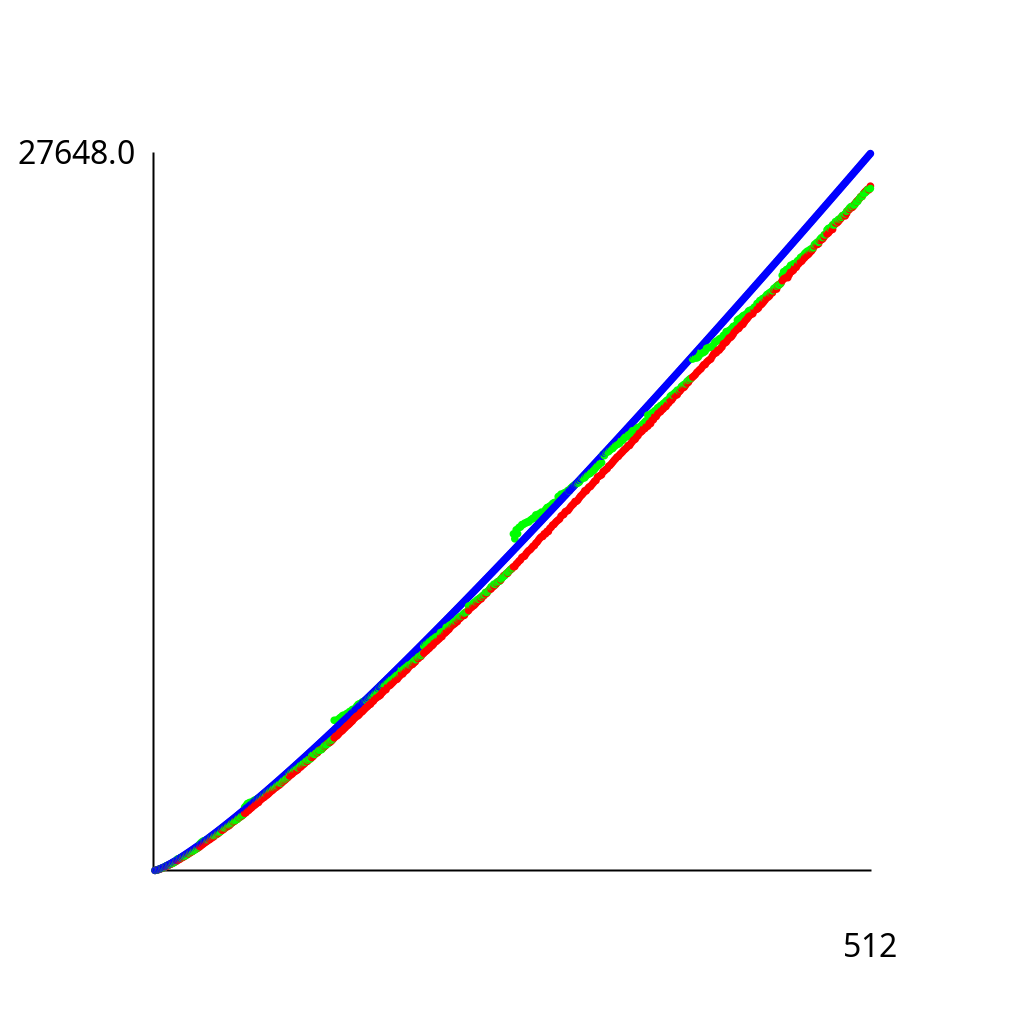
\includegraphics[width=0.6\textwidth]{mergesort-array-access-cost-plot}
			\caption{Plot for Exercise 2.2.6; top-down mergesort in red, bottom-up mergesort in green,
			and the $6n\lg n$ bound in blue}
			\label{ex:6}
		\end{figure}
		See Figure~\ref{ex:6}.
	\end{sol}
	\begin{ex}{7}
		Show that the number of compares used by mergesort is monotonically increasing,
		meaning $C(n+1)>C(n)$ for all $n>0$.
	\end{ex}
	\begin{sol}
		The result actually depends on the contents of the array. For example,
		if an array is not sorted with $n$ elements and another array \emph{is} sorted
		and has $n+1$ elements, then the number of compares is smaller for the
		second array. Therefore, I do not think this is true in general, and I need
		more information to understand what conditions makes this true.
	\end{sol}
	\begin{ex}{8}
		Suppose that Algorithm 2.4 is modified to skip the call on \texttt{merge()} whenever
		\texttt{a[mid] <= a[mid+1]}. Prove that the number of compares used to mergesort
		a sorted array is linear.
	\end{ex}
	\begin{sol}
		\begin{proof}
			With this modification, the algorithm does one compare for each recursive call.
			Let $k=\lfloor \lg(n) \rfloor$. If $i$ is an integer between $0$ and $k$ (inclusive),
			then $i$, then $i$ represents the recursion depth of merge sort. In particular,
			$i=0$ is the initial call, and the $i$th level has $2^i$ recursive calls.
			The total number of recursive calls, and hence the total number of compares, is
			bounded by
			\begin{align*}
				\sum_{i=0}^{k}2^i&=2^{k+1}-1\\
				&=2\cdot 2^k-1\\
				&=2\cdot 2^{\lfloor \lg n\rfloor } -1\\
				&\leq 2\cdot 2^{\lg n +1}- 1\\
				&=4n-1
			\end{align*}
			Similarly it is bounded below by $\sum_{i=0}^{k-1}2^i$. We conclude that it is linear.
		\end{proof}
	\end{sol}
	\begin{ex}{9}
		Use of a static array like \texttt{aux[]} is inadvisable in library software because
		multiple clients might use the class concurrently. Give an implementation of \texttt{Merge}
		that does not use a static array. Do \emph{not} make \texttt{a[]} local to \texttt{merge()}
		(see the Q \& A for this section).
		\emph{Hint}: Pass the auxiliary array as an argument to the recursive \texttt{sort()}.
	\end{ex}
	\begin{sol}
		See the \texttt{com.segarciat.algs4.ch2.sec2.ex09.Merge} class.
	\end{sol}
	\begin{ex}{10}
		\emph{Faster merge}. Implement a version of \texttt{merge()} that copies the second half of
		\texttt{a[]} to \texttt{aux[]} in \emph{decreasing order} and then does the merge back to \texttt{a[]}.
		This change allows you to remove the code to test that each of the halves has been
		exhausted from the inner loop. \emph{Note}: The resulting sort is not stable
		(see page 341).
	\end{ex}
	\begin{sol}
		See the \texttt{com.segarciat.algs4.ch2.sec2.ex10.FasterMerge} class.
	\end{sol}
	\begin{ex}{11}
		\emph{Improvements}. Implement the three improvements to mergesort that are described
		in the text on page 275: Add a cutoff for small subarrays, test whether the array
		is already in order, and avoid the copy by switching arguments in the recursive code.
	\end{ex}
	\begin{sol}
		See the \texttt{com.segarciat.algs4.ch2.sec3.ex11.MergeImproved} class.
	\end{sol}
	\begin{ex}{12}
		\emph{Sublinear extra space}. Develop a merge implementation that reduces the extra
		space requirement to $\max(n/m)$, based on the following idea: Divide the array into
		$n/m$ blocks of size $m$ (for simplicity in this description, assume that $n$ is a
		multiple of $m$). Then,
		\begin{enumerate}[label=(\roman*)]
			\item Considering the blocks as items with their first key as the sort key,
			sort them using selection sort; and
			\item Run through the array merging the first block with the second, then the
			second with the third, and so forth.
		\end{enumerate}
	\end{ex}
	\begin{sol}
		TODO.
	\end{sol}
	\begin{ex}{13}
		\emph{Lower bound for average case}. Prove that the expected number of compares
		used by any compared-based sorting algorithm must be at least $n\lg n$
		(assuming that all possible orderings of the input are equally likely).
		\emph{Hint}: The expected number of compares is at least the external path
		length of the compare tree (the sum of the lengths of the paths from the root
		to all leaves), which is minimized when it is balanced.
	\end{ex}
	\begin{sol}
		TODO.
	\end{sol}
	\begin{ex}{14}
		\emph{Merging sorted queues}. Develop a static method that takes two queues of sorted
		items as arguments and returns a queue that results from merging the the queues
		into sorted order.
	\end{ex}
	\begin{sol}
		See the \texttt{com.segarciat.algs4.ch2.sec2.ex14.MergeQueues} class.
	\end{sol}
	\begin{ex}{15}
		\emph{Bottom-up queue mergesort}. Develop a bottom-up mergesort implementation based
		on the following approach: Given $n$ items, create $n$ queues, each containing one
		of the items. Create a queue of the $n$ queues. Then, repeatedly apply the merging
		operation of Exercise 2.2.14 to the first two queues and reinsert the merged queue
		at the end. Repeat until the queue of queues contains only one queue.
	\end{ex}
	\begin{sol}
		See the\texttt{com.segarciat.algs4.ch2.sec2.ex15.MergeBUQueue} class.
	\end{sol}
	\begin{ex}{16}
		\emph{Natural mergesort}. Write a version of bottom-up mergesort that takes advantage
		of order in the array by proceeding as follows each time it needs to find
		two arrays to merge: find a sorted subarray (by incrementing a pointer until
		finding an entry that is smaller than its predecessor in the array), then find
		the next, then merge them. Analyze the running time of this algorithm in terms
		of the array length and the number of maximal increasing sequences in the array.
	\end{ex}
	\begin{sol}
		See the \texttt{com.segarciat.algs4.ch2.sec2.ex16.NaturalMergeBU} class.
		Let $n$ be the length of the array we are sorting. In the worst case,
		there's $n$ increasing sequences, because the array may be sorted in
		reverse with distinct elements. In that case, there are $n-1$ merges,
		in each with an array of size $1$ for the second array.
		Because the \texttt{merge()} operation is linear in the size of the
		input arrays (given that it must copy all elements), the performance
		degrades to quadratic in this case. For example, it would require copying
		$1$ element, then $2$, then $3$, and so on until the last merge where
		it has to copy $n-1$ elements. In general, if there are $k$ maximal increasing
		sequences in the array, then each pass through the array decreases the number
		of maximal increasing sequences by $1$, and the algorithm stops when only
		one remains; at that point, the array is sorted. The cost is then $k$ merges.
	\end{sol}
	\begin{ex}{17}
		\emph{Linked-list sort}. Implement a natural mergesort for linked lists. (This is the
		method of choice for sorting linked lists because it uses no extra space and
		is guaranteed to be linearithmic).
	\end{ex}
	\begin{sol}
		See the \texttt{com.segarciat.algs4.ch2.sec2.ex17.LinkedListNaturalMergesort} class.
	\end{sol}
	\begin{ex}{19}
		\emph{Inversions}. Develop and implement a linearithmic algorithm for computing
		the number of inversions in a given array (the number of exchanges that
		would be performed by insertion sort for that array --- see Section 2.1).
		This quantity is related to the \emph{Kendall tau distance}; see Section 2.5.
	\end{ex}
	\begin{sol}
		See the \texttt{com.segarciat.algs4.ch2.sec2.ex19.Inversions} class.
	\end{sol}
	\begin{ex}{20}
		\emph{Index sort}. Develop and implement a version of mergesort that does not
		rearrange the array, but returns an \texttt{int[]} array `perm` such that \texttt{perm[i]}
		is the index of the $i$th smallest entry in the array.
	\end{ex}
	\begin{sol}
		See the \texttt{com.segarciat.algs4.ch2.sec2.ex20.IndexSort} class.
	\end{sol}
	\begin{ex}{21}
		\emph{Triplicates}. Given three lists of $n$ names each, devise a linearithmic
		algorithm to determine if there is a name common to all three lists,and if so,return
		the lexigraphically first such name.
	\end{ex}
	\begin{sol}
		See the \texttt{com.segarciat.algs4.ch2.sec2.ex21.Triplicates} class.
	\end{sol}
	\begin{ex}{22}
		\emph{3-way mergesort}. Suppose instead of dividing in half at each step, you
		divide into thirds,s ort each  third, and combine using a 3-way merge. What is
		the order of growth of the overall running time of this algorithm?
	\end{ex}
	\begin{sol}
		If we make a tree of the recursive calls implied by this algorithm, rooted
		at the initial call, then we get a trinary three, and the height of the
		tree is about $\log_3(n)$, where $n$ is the number of elements in the
		array. At each recursive call when having a size of $N\leq n$, the
		merge takes up at most $N$ comparisons. We could write a recursive formula
		similar to the one for (binary) mergesort:
		\begin{align*}
			C(n)\leq C(\lceil n / 3\rceil) + C(\lceil n / 3 \rceil) + C(\lfloor n / 3 \rfloor ) + n
		\end{align*}
		On the right-hand side, the first two are upper bounds on the cost for sorting the
		first two thirds, the third term is the cost of compares for sorting the last third,
		and an upper bound for the $n$ is the cost of the merge. I conjecture (but
		will not prove) that the resulting algorithm is thus linearithmic, because
		it will likely use $\sim n\log_3n$ compares.
	\end{sol}
	\begin{ex}{23}
		\emph{Improvements}. Run empirical studies to evaluate the effectiveness of each of the
		three improvements to mergesort that are described in the text (see Exercise 2.2.11).
		Also, compare the performance of the merge implementation given in the text with the
		merge described in Exercise 2.2.10. In particular, empirically determine the best value
		of the parameter that decides when to switch to insertion sort for small subarrays.
	\end{ex}
	\begin{sol}
		See \texttt{com.segarciat.algs4.ch2.sec2.ex23}. In summary, all of these improvements
		are observed, with the least prominent being the improvement that skips the
		merge for arrays that are already sorted, though in that case, it still
		performs around linearithmically. Of course, the added bonus is that it is
		linear for sorted arrays. For the insertion cutoff value, I found that on my
		system I get an improvement of about $200\%$ for a \texttt{CUTOFF} of about $63$.
		My implementation\texttt{MergeImproved} from Exercise 2.2.11 that combines all
		three improvements leads to a performance improvement of about $300\%$, or so
		I observed..
	\end{sol}
	\pagebreak
	\printbibliography
\end{document}